\documentclass[ALICE,manyauthors]{cernphprep}
\usepackage[comma,square,numbers,sort&compress]{natbib}
\usepackage{hyperref}
\usepackage{lineno}
\usepackage{xspace}
\usepackage[table]{xcolor}
\usepackage{siunitx}
\sisetup{binary-units=true}
\sisetup{load-configurations = abbreviations}
\linenumbers

%%%%%%%%%%%%%%%%%%%%%%%%%%%%%%%%%%%%%%%%%%%%%%%%%%
% These are some new commands that may be useful 
% for paper writing in general. If other newcommands
% are needed for your specific paper, please feel 
% free to add here. 
%
% The currently available commands are organized in: 
% 1) Systems
% 2) Quantities
% 3) Energies and units
% 4) Detectors
% 5) particle species 
%%%%%%%%%%%%%%%%%%%%%%%%%%%%%%%%%%%%%%%%%%%%%%%%%%

% 1) SYSTEMS 
\newcommand{\pp}           {pp\xspace}
\newcommand{\ppbar}        {\mbox{$\mathrm {p\overline{p}}$}\xspace}
\newcommand{\XeXe}         {\mbox{Xe--Xe}\xspace}
\newcommand{\PbPb}         {\mbox{Pb--Pb}\xspace}
\newcommand{\pA}           {\mbox{pA}\xspace}
\newcommand{\pPb}          {\mbox{p--Pb}\xspace}
\newcommand{\AuAu}         {\mbox{Au--Au}\xspace}
\newcommand{\dAu}          {\mbox{d--Au}\xspace}

% 2) QUANTITIES 
\newcommand{\s}            {\ensuremath{\sqrt{s}}\xspace}
\newcommand{\snn}          {\ensuremath{\sqrt{s_{\mathrm{NN}}}}\xspace}
\newcommand{\pt}           {\ensuremath{p_{\rm T}}\xspace}
\newcommand{\meanpt}       {$\langle p_{\mathrm{T}}\rangle$\xspace}
\newcommand{\ycms}         {\ensuremath{y_{\rm CMS}}\xspace}
\newcommand{\ylab}         {\ensuremath{y_{\rm lab}}\xspace}
\newcommand{\etarange}[1]  {\mbox{$\left | \eta \right |~<~#1$}}
\newcommand{\yrange}[1]    {\mbox{$\left | y \right |~<~#1$}}
\newcommand{\dndy}         {\ensuremath{\mathrm{d}N_\mathrm{ch}/\mathrm{d}y}\xspace}
\newcommand{\dndeta}       {\ensuremath{\mathrm{d}N_\mathrm{ch}/\mathrm{d}\eta}\xspace}
\newcommand{\avdndeta}     {\ensuremath{\langle\dndeta\rangle}\xspace}
\newcommand{\dNdy}         {\ensuremath{\mathrm{d}N_\mathrm{ch}/\mathrm{d}y}\xspace}
\newcommand{\Npart}        {\ensuremath{N_\mathrm{part}}\xspace}
\newcommand{\Ncoll}        {\ensuremath{N_\mathrm{coll}}\xspace}
\newcommand{\dEdx}         {\ensuremath{\textrm{d}E/\textrm{d}x}\xspace}
\newcommand{\RpPb}         {\ensuremath{R_{\rm pPb}}\xspace}

% 3) ENERGIES, UNITS
\newcommand{\nineH}        {$\sqrt{s}~=~0.9$~Te\kern-.1emV\xspace}
\newcommand{\seven}        {$\sqrt{s}~=~7$~Te\kern-.1emV\xspace}
\newcommand{\twoH}         {$\sqrt{s}~=~0.2$~Te\kern-.1emV\xspace}
\newcommand{\twosevensix}  {$\sqrt{s}~=~2.76$~Te\kern-.1emV\xspace}
\newcommand{\five}         {$\sqrt{s}~=~5.02$~Te\kern-.1emV\xspace}
\newcommand{\twosevensixnn}{$\sqrt{s_{\mathrm{NN}}}~=~2.76$~Te\kern-.1emV\xspace}
\newcommand{\fivenn}       {$\sqrt{s_{\mathrm{NN}}}~=~5.02$~Te\kern-.1emV\xspace}
\newcommand{\LT}           {L{\'e}vy-Tsallis\xspace}
\newcommand{\GeVc}         {Ge\kern-.1emV/$c$\xspace}
\newcommand{\MeVc}         {Me\kern-.1emV/$c$\xspace}
\newcommand{\TeV}          {Te\kern-.1emV\xspace}
\newcommand{\GeV}          {Ge\kern-.1emV\xspace}
\newcommand{\MeV}          {Me\kern-.1emV\xspace}
\newcommand{\GeVmass}      {Ge\kern-.2emV/$c^2$\xspace}
\newcommand{\MeVmass}      {Me\kern-.2emV/$c^2$\xspace}
\newcommand{\lumi}         {\ensuremath{\mathcal{L}}\xspace}

% 4) DETECTORS 
\newcommand{\ITS}          {\rm{ITS}\xspace}
\newcommand{\TOF}          {\rm{TOF}\xspace}
\newcommand{\ZDC}          {\rm{ZDC}\xspace}
\newcommand{\ZDCs}         {\rm{ZDCs}\xspace}
\newcommand{\ZNA}          {\rm{ZNA}\xspace}
\newcommand{\ZNC}          {\rm{ZNC}\xspace}
\newcommand{\SPD}          {\rm{SPD}\xspace}
\newcommand{\SDD}          {\rm{SDD}\xspace}
\newcommand{\SSD}          {\rm{SSD}\xspace}
\newcommand{\TPC}          {\rm{TPC}\xspace}
\newcommand{\TRD}          {\rm{TRD}\xspace}
\newcommand{\VZERO}        {\rm{V0}\xspace}
\newcommand{\VZEROA}       {\rm{V0A}\xspace}
\newcommand{\VZEROC}       {\rm{V0C}\xspace}
\newcommand{\Vdecay} 	   {\ensuremath{V^{0}}\xspace}

% 4) PARTICLE SPECIES 
\newcommand{\ee}           {\ensuremath{e^{+}e^{-}}} 
\newcommand{\pip}          {\ensuremath{\pi^{+}}\xspace}
\newcommand{\pim}          {\ensuremath{\pi^{-}}\xspace}
\newcommand{\kap}          {\ensuremath{\rm{K}^{+}}\xspace}
\newcommand{\kam}          {\ensuremath{\rm{K}^{-}}\xspace}
\newcommand{\pbar}         {\ensuremath{\rm\overline{p}}\xspace}
\newcommand{\kzero}        {\ensuremath{{\rm K}^{0}_{\rm{S}}}\xspace}
\newcommand{\lmb}          {\ensuremath{\Lambda}\xspace}
\newcommand{\almb}         {\ensuremath{\overline{\Lambda}}\xspace}
\newcommand{\Om}           {\ensuremath{\Omega^-}\xspace}
\newcommand{\Mo}           {\ensuremath{\overline{\Omega}^+}\xspace}
\newcommand{\X}            {\ensuremath{\Xi^-}\xspace}
\newcommand{\Ix}           {\ensuremath{\overline{\Xi}^+}\xspace}
\newcommand{\Xis}          {\ensuremath{\Xi^{\pm}}\xspace}
\newcommand{\Oms}          {\ensuremath{\Omega^{\pm}}\xspace}
\newcommand{\degree}       {\ensuremath{^{\rm o}}\xspace}

\begin{document}

\begin{titlepage}
% the dates below correspond to CERN approval
% please don't touch: EB chairs will take care
\PHyear{XXXX}       % required, will be obtained from CERN
\PHnumber{XXX}      % required, will be obtained from CERN
\PHdate{Day Month}  % required, will be obtained from CERN

%%% Put your own title + short title here:
\title{ALICE upgrades during the LHC long-shutdown 2}
\ShortTitle{ALICE LS2 upgrades}   % appears on left page headers

%%% Do not change the next lines
\Collaboration{ALICE Collaboration\thanks{See Appendix~\ref{app:collab} for the list of collaboration members}}
\ShortAuthor{ALICE Collaboration} % appears on right page headers, do not change

\begin{abstract}
In this article, we discuss the ALICE upgrades during the LHC long-shutdown 2.
\end{abstract}
\end{titlepage}

\setcounter{page}{2} %please do not remove this line

\tableofcontents
\listoffigures

\nocite{EBGuidelineEditing}

\section{Introduction (Marco, Jochen; 8 p.)}

A Large Ion Collider Experiment (ALICE) has been proposed and built to study
the properties of the Quark-Gluon Plasma in hadronic collisions at the Large
Hadron Collider at CERN~\cite{Aamodt:2008zz}. The design was driven by the
requirement to cope with the high multiplicities in central \PbPb collisions
and provide a complete reconstruction of the events, including particle
identification over a wide \pt range.

The experimental setup consists of a central barrel contained in a solenoidal
magnet ($B = 0.5~\mathrm{Tesla}$) and a forward muon-system with a dipole magnet
providing $3~\mathrm{Tm}$, see Fig.~\ref{fig:alice_run2}. Until the end of Run~2,
the central barrel contained an Inner Tracking System (ITS) with two layers of
Silicon Pixel Detectors (SPD), two layers of Silicon Drift Detectors (SDD), and
two layers of Silicon Strip Detectors (SSD). In radial direction, it is followed
by a Time Projection Chamber (TPC) covering the radii from 0.5~m to 2.5~m over a
length of 7~m.
The central barrel detector system is designed for efficient trakcing in the high track-density environment of heavy ion collisions, covering momenta from low to high \pt{} with good hadron and electron identification capabilities.

The forward muon detectors cover the rapidity range $2.5 < \eta < 4.0$ (tbc) and use a system of absobers to remove hadrons and idensify muons.
The background of secondary muons from pion and kaon decays in the muon system is small at high pt, thanks to the so-called 'muon plug' absorber, which is placed at $z = xx$ cm from the interaction point.

The forward muon detectors cover the rapidity range $2.5 < \eta < 4.0$ (tbc) and use a system of absobers to remove hadrons and idensify muons.
The background of secondary muons from pion and kaon decays in the muon system is small at high pt, thanks to the so-called 'muon plug' absorber, which is placed at $z = xx$ cm from the interaction point.

\subsection{Tracking}

The ALICE detector system is designed for high-efficiency tracking with excellent two-track separation in high-multiplicity events. The efficient tracking extends down to low $\pt \approx \SI{100}{\mega\eV\per\clight}$ (todo: check canonical value) which is important to access the kinematic range where thermal production from the QGP plays a role and to reconstruct weak and strong decays.
Similarly, the two-track resolution is important for decay reconstruction, as well as correlation measurements that reveal the space-time structure of particle production ('femtoscopy') and probe interactions between hadrons as well as jet structure measurements.

Give some key performance numbers: momentum resolution and impact parameter resolution...

\subsection{Tracking performance}

The ALICE detector system is designed for high-efficiency tracking with excellent two-track separation in high-multiplicity events. The efficient tracking extends down to low $\pt \approx 100$ MeV/$c$ (todo: check canonical value) which is important to access the kinematic range where thermal production from the QGP plays a role and to reconstruct weak and strong decays.
Similarly, the two-track resolution is important for decay reconstruction, as well as correlation measurements that reveal the space-time structure of particle production ('femtoscopy') and probe interactions between hadrons as well as jet structure measurements.

Give some key performance numbers: momentum resolution and impact parameter resolution...

\begin{figure}
\centering
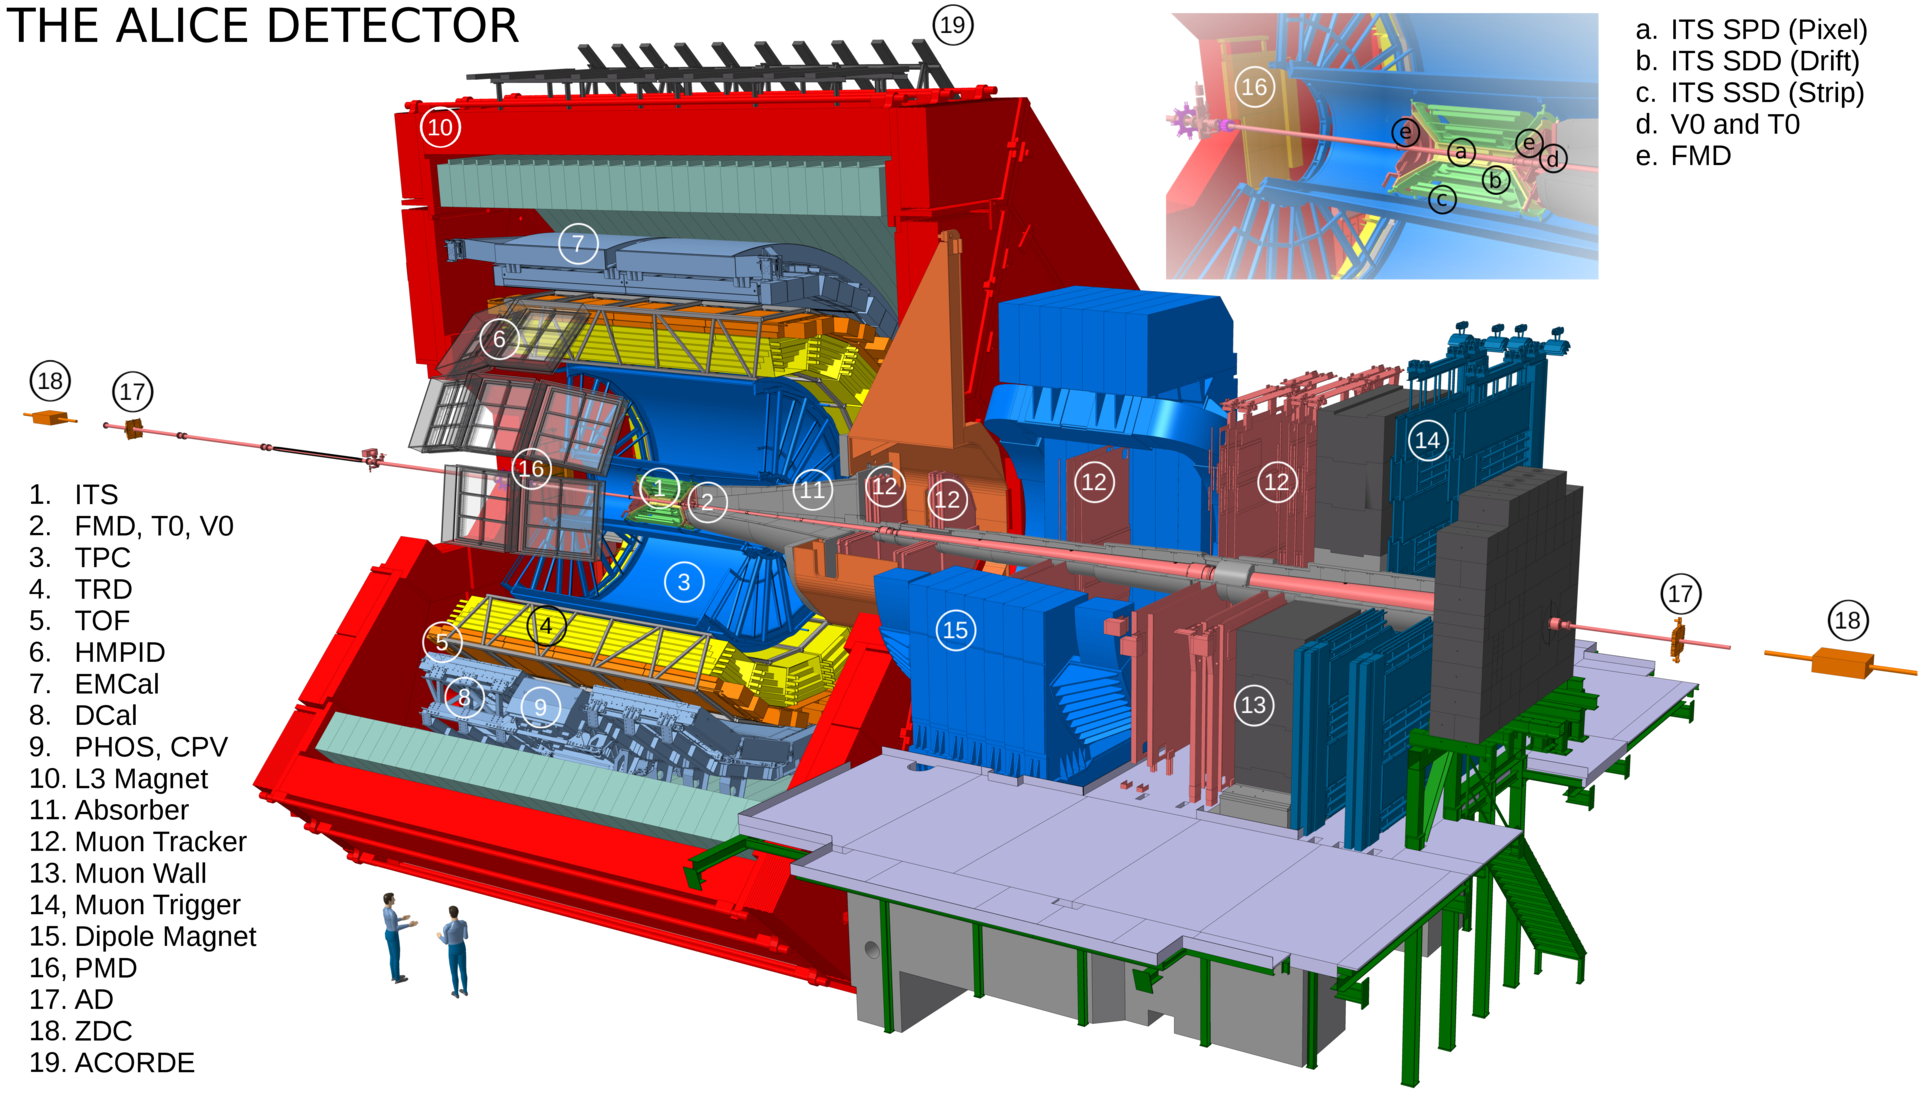
\includegraphics[width=.7\textwidth]{intro/2017-May-11-ALICE_RUN2_labels_HD}
\caption{Detector setup in Run 2}
\label{fig:alice_run2}
\end{figure}

\begin{figure}
\centering
\caption{tracking efficiency}
\label{fig:trk_eff}
\end{figure}

\begin{figure}
\centering
\caption{tracking \pt resolution}
\label{fig:trk_res}
\end{figure}

\subsection{Calorimetry}

\subsection{Particle identification}

\begin{figure}
\centering
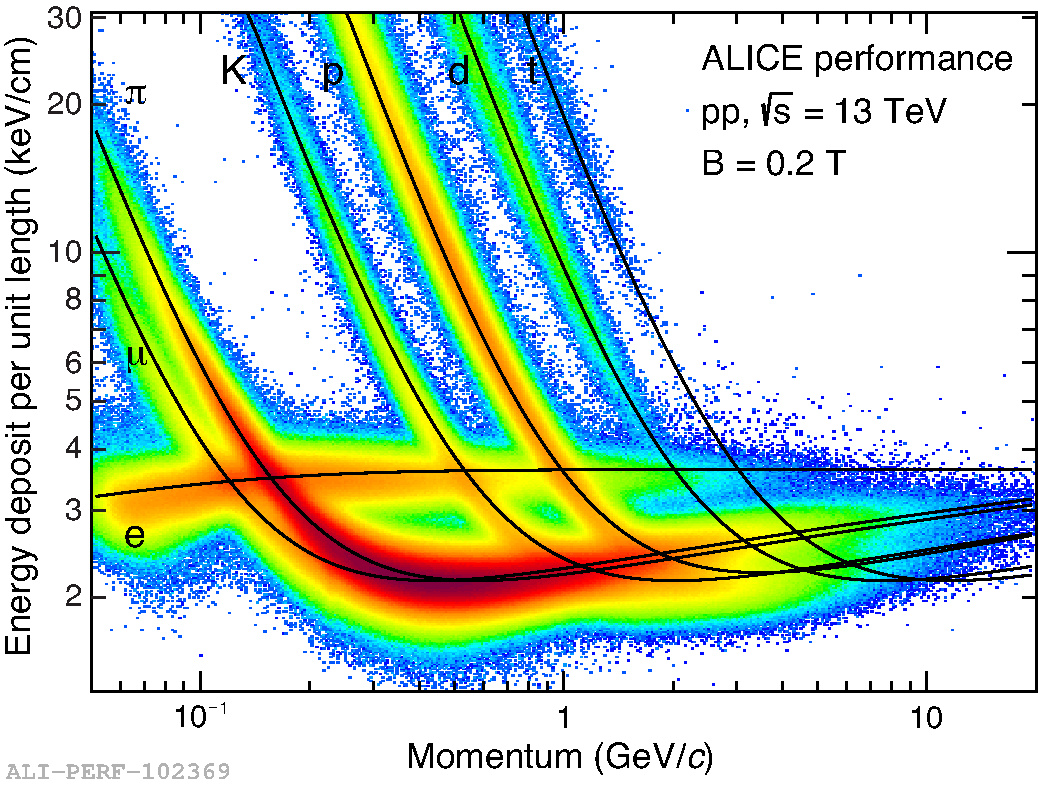
\includegraphics[width=.7\textwidth]{intro/2018-Jul-23-TPC_dEdx_2T_151003_color}
\caption{TPC dE/dx}
\label{fig:tpc_dedx}
\end{figure}

\subsection{Event characterization and selection}

\subsection{Forward spectrometer}

\subsection*{Run1/2 performance highlights (examples)}

cite performance paper~\cite{Abelev:2014ffa}, possibly also detector papers

discuss performance
\begin{itemize}
\item particle identification and relevant detectors
\item secondary vertex resolution
\item data sets (rate/integrated luminosity)
\end{itemize}

Data was recorded throughout the
running of the LHC in Run 1 and 2 exploiting a variety of collision systems and
energies, see Tab.~\ref{tab:datasets}.

\begin{figure}
\centering
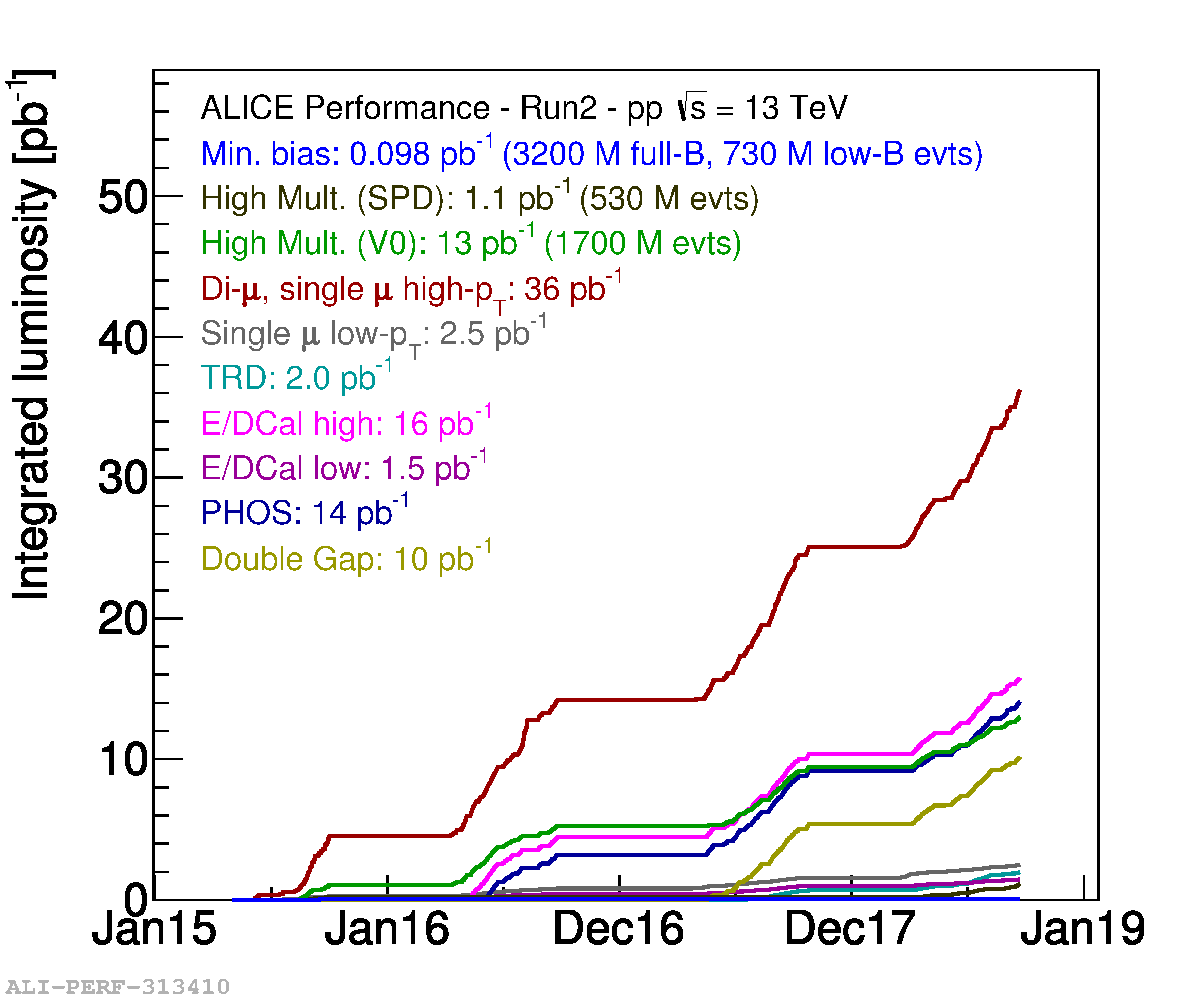
\includegraphics[width=.45\textwidth]{intro/2019-01-17-2019-01-17-lumi_Run2_pp13TeV}
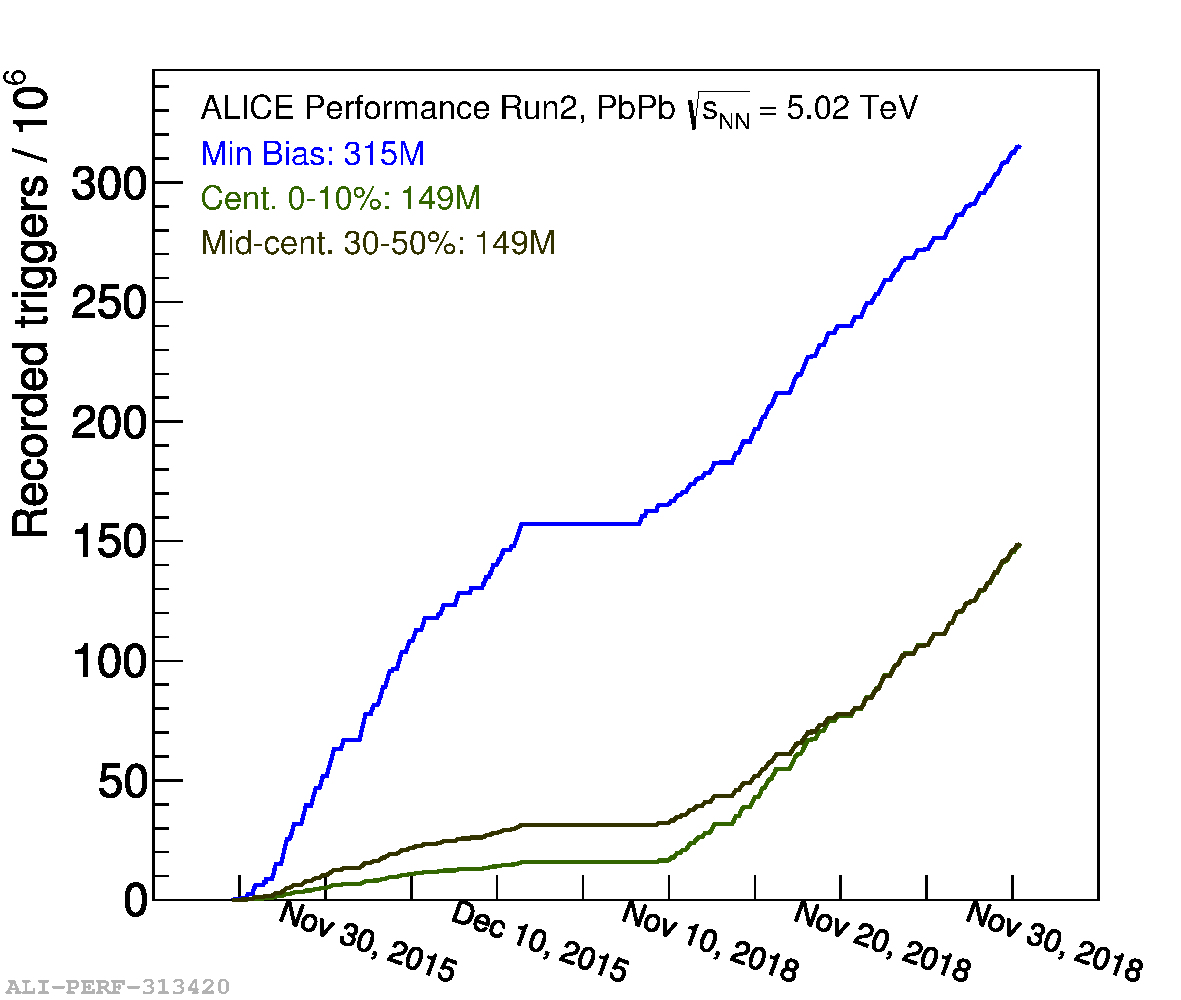
\includegraphics[width=.45\textwidth]{intro/2019-01-17-2019-01-17-stat_Run2_PbPb}
\caption{integrated lumi}
\label{fig:lumi_run2}
\end{figure}

\begin{table}
  \centering
  \begin{tabular}{lrrr}
    \multicolumn{1}{c}{system}
    & \multicolumn{1}{c}{$\snn~(\mathrm{\TeV})$}
    & \multicolumn{1}{c}{$L_\mathrm{MB}$}
    & \multicolumn{1}{c}{$L_\mathrm{insp}$}\\
    \hline \hline
    \pp & 0.9 & & $\sim \SI{200}{\micro \barn^{-1}}$\\
        & 2.76 & & $\sim 100~\mathrm{nb}^{-1}$\\
        & 5.02 & & $\sim 1.3~\mathrm{pb}^{-1}$\\
        & 7 & & $\sim 1.5~\mathrm{pb}^{-1}$\\
        & 8 & & $\sim 2.5~\mathrm{pb}^{-1}$\\
        & 13 & & $\sim 25~\mathrm{pb}^{-1}$\\
    \pPb{} & 5.02 & & $\sim 15 + 3~\mathrm{nb}^{-1}$\\
           & 8.16 & & $\sim 25~\mathrm{nb}^{-1}$\\
    \XeXe{} & 5.44 & & $\sim 0.3~\mu\mathrm{b}^{-1}$\\
    \PbPb{} & 2.76 & & $\sim 75~\mu\mathrm{b}^{-1}$\\
            & 5.02 & & $\sim 0.25 + 1~\mathrm{nb}^{-1}$\\
    \hline
  \end{tabular}
  \caption{ALICE datasets from LHC Run 1 and 2}
  \label{tab:datasets}
\end{table}


\section{Upgrade objectives, motivations and goals (10 p.)}

The ALICE detector has undergone a major upgrade during the Long Shutdown 2 of the LHC, 2019-2021.
The main goal of the upgrade is to improve the performance for rare, untriggered signals: the production of open heavy flavor mesons and baryons which serve as important 'trace particles' that probe both early and late time dynamics in the collision, as well as electron-positron pairs which measure the temperature of the hot and dense Quark Gluon Plasma produced in the collision, as well as effects related to chiral symmetry restoration.
To achieve this, the full Inner Tracking System has been replaced with a new system based on monolithic active pixel sensors with a better spatial resolution than the previous ITS, as well as a lower material budget, to further improve the spatial resolution and reduce the background from photon conversions. The readout chambers of the TPC have been replaced with multi-foil GEM chambers to reduce the ion backflow and allow continuous readout of the TPC.
In the forward direction, the new Muon Forward Tracker (MFT) is a silicon pixel tracker that provides accurate pointing for muon tracks, to identify quarkonia from beauty decays.
The trigger and data acquisition systems have been completely redesigned and replaced with an online processing system that performs important parts of the reconstruction, to reduce the data rate while keeping information on all events and primary tracks. The readout electronics of several sub-detectors has been replaced to provide larger readout rates than were previously possible and to be compatible with the new online data acquisition and processing system. 

\subsection{Physics performance (Marco, Jochen)}

The physics programme motivating the upgrade was first established in the Letter of Intent~\cite{Abelevetal:2014cna} and the individual Technical Design Reports. Later, it was scrutinized by Working Group 5 of \dots leading to a report~\cite{Citron:2018lsq}, which summarizes the potential of heavy-ion physics at the LHC in Run 3 and 4 across all the LHC experiments. This report identified core areas of interests and the corresponding measurements and observables. The precise measurement of the long-wavelength behaviour, i.e. the macroscopic fluid-like evolution of a high-density and high-temperature system, allows us to draw conclusions on the phase transition as well as material properties of a deconfined state of matter. Access to the microscopic parton dynamics which underlies the QGP allows us to understand the fundamental degrees of freedom and interactions in a deconfined state. A further goal is to systematicaly study particle production across collision systems in order to assess the validity of the fluid description and the role of collectivity. Finally, the precise measurement of nuclear parton densities over a wide $(x, Q^2)$ range is fundamental to constrain the initial conditions.

\subsubsection{Heavy-flavour and quarkonia production}

\subsubsection{Low-mass dileptons}

\subsubsection{Jets}

\subsubsection{Nuclear states}

hyper nuclei

\subsubsection{Small systems}

particle production and energy loss

\subsubsection{small $x$}

nuclear PDFs

\subsubsection{Requirements}
\label{sec:physics_motivation}

These physics goals translate to requirements on operational conditions and detector systems. While the details shall be discussed in the next section, we will only summarise the essence here. The high interaction rates needed to accumulate enough integrated luminosity (up to 50 kHz \PbPb{} and up to 1 MHz \pp{}), require the operation of the TPC without gating and, thus, with significantly reduced ion back flow. The precise reconstruction of secondary vertices can be achieved by an Inner Tracking System, with a smaller radius of the innermost layer and with a better position resolution in each layer. Probes which only show as a small signal on top of large combinatorial background, cannot be triggered and require large statistics to be analysed. This implies the processing of un-preselected (untriggered) events from the continuosly read-out TPC. In addition, the performance of particle identification must not be deteriorated in order to extract significant measurements in environments of large combinatorial background.

%\subsection{System design (Werner, Alex)}



\subsection{System design - ALICE read-out architecture}

As a consequence of the increase of the Pb--Pb interaction rate to 50 kHz in average 5 TPC drift time periods ($\approx 100\; \mu s$) are overlapping at any given moment. That means that the TPC permanently will contain useful data which requires continuous, trigger-less read-out. In addition, the Pb--Pb event topology would only allow adaptation of the actual data throughput to the available read-out data bandwidth as it has been done in run 1 and 2 and not a selection based on event topology. The ALICE read-out system upgrade overcomes this limit by increasing the read-out bandwidth and registering all interactions without event selection by providing a trigger-less and continuous read-out mode. Nevertheless, the ALICE read-out system features dedicated trigger detectors which are read out in continuous mode to facilitate reconstruction and commissioning. Upgraded Trigger detectors are the fast interaction trigger (FIT) indicating the presence and centrality of an interaction, the zero degree calorimeter (ZDC) providing information @ and the time of flight detector (TOF) serving as cosmic ray trigger for commissioning purposes. 

In addition to the nominal continuous read-out mode, all upgraded detector systems support triggered read-out mode. In this mode only data from selected interactions are being retained by the read-out electronics. Triggered read-out mode allows adaptation of the ALICE read-out data throughput during commissioning or dedicated calibrations runs where the data bandwidth exceeds nominal conditions.

The upgraded ALICE detector features a number of legacy detectors (CPV, EMCAL, PHOS, TRD) which are not read out in in continuous mode but will need a hardware trigger signal provided by the FIT detector to indicate when an interaction took place. The read-out data of these detectors are merged with the read-out data from the continuously read out detectors. 

Some of the detectors (EMCAL, PHOS) provide a hardware trigger signal. The trigger outputs of all trigger detectors (FIT, ZDC, EMCAL, PHOS) are fed into the central trigger system (CTS) for the afore mentioned commissioning and calibration runs but also for dedicated special runs using the EMCAL and PHOS triggers.

In order to synchronise the continuous data stream in all read-out branches and also to give the continuous data a structure for reconstruction the read-out stream is divided in so-called time frames (TF) of programmable length with a nominal duration of 11 ms. Each TF is divided in heart beat frames (HBF) with a length corresponding to an LHC orbit of $\approx 89.4\; \mu s$. Fig. \ref{fig_ro:tf_hbf_structure} shows an illustration of this structure. In continuous mode all detector data are forwarded, whereas in triggered mode only data from interactions with a positive trigger signal are retained. In both cases the data are formatted in HBFs.

Fig. \ref{fig_ro:ro_architecture}  shows the ALICE read-out system and its three detector read-out groups \cite{TDR, run34note}. In the first group which contains all upgraded detectors with the exception of CPV, ITS and MFT, the central trigger system (CTS) receives the machine clock and trigger inputs signals in the central trigger processor (CTP) and fan-outs out the signals via the local trigger units (LTU) to the common read-out units (CRU) using bi-directional TTC-PON links. The CRUs are standardised PCIe and FPGA based optical I/O processor modules (see section \ref{sec:flp}) which forward the timing and trigger information to the front-end electronics on bi-directional optical GBT links \cite{ro:GBT} initiating the detector read-out. The detector data are sent to the CRUs  from where the HBF data are shipped via the PCIe interface to the first level processors (FLP) in the O2 farm. The FLPs prepares the Sub-Time Frames (STF) merging all HBFs of one TF of the connected detectors and ships them to the event processing nodes (EPN). There the STFs of all sub-detectors are merged into a TF. 

The second group contains the CPV, the ITS and MFT detectors which fully support the upgraded continuous read-out strategy and is identical to the first group, with the exception that the front-end requires a trigger signal indicating the presence of an interaction with short latency of 1.6 us. As the propagation delay from the CTS in the cavern via the CRU on surface back to the front-end electronics in the cavern would be too long, a parallel and shorter timing and trigger signal path using the GBT protocol is established directly from the CTS to the ITS/MFT front-ends. 

The third group contains legacy detectors which are not upgraded and are read out via legacy read-out cards C-RORC  \cite{ro:CRORC} located in FLPs. They receive the clock and trigger signals via the legacy TTC system \cite{ro:TTC}. Table \ref{table_ro:datathroughput} shows a summary of the data throughputs and ? for each detector (should that information be added to Pierres table?).

The CTS controls the read-out of the sub-detectors and provides in addition to the clock the heart beat (HB) triggers to the CRU and the connected front-end electronics. The HB triggers define whether the interactions contained in a given HBF are supposed to be registered (HB accept, HBa) or whether the data from the corresponding HBF should be deleted (HB reject, HBr) in the CRU. The CRUs in turn give information to the CTS whether a given HBF has been successfully transported to the FLP or whether HBF data packets are missing or a buffer overflow occurred (HB acknowledge, HBack). 
For each HBF the CTS evaluates and summarises all HBack messages from all CRUs into the  HBF decision message. The HBF decision messages is sent via the CRU to the FLP indicating whether a given HBF is considered useful for data storage or whether it should be deleted. This data flow control signal scheme is illustrated in fig. \ref{fig_ro:control_signals} and allows an adaptation of the data throughput in the read-out system to the available bandwidth during commissioning or optimisation of detector read-out parameters. In nominal conditions, the system allows immediate monitoring of the read-out components and immediate reaction.

\begin{figure*}[hbtp]
  \begin{center}
    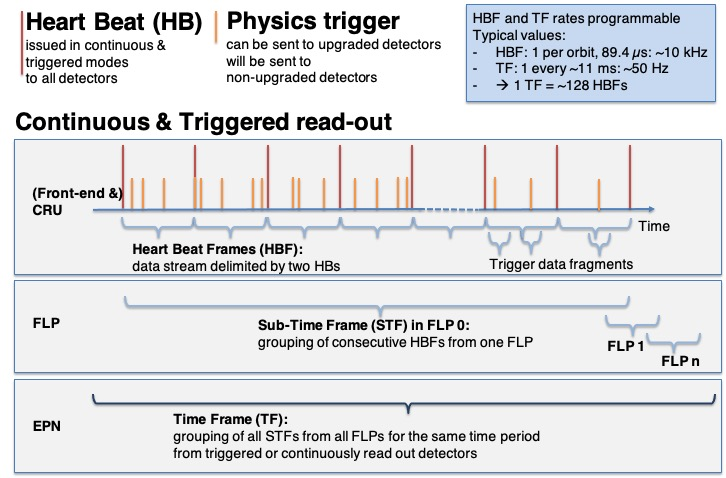
\includegraphics[width=1.\textwidth]{../fig/cru/tf_hbf_structure.jpg}
  \end{center}
  \caption{TF and HBF structure: additional info will be added here@}
  \label{fig_ro:tf_hbf_structure}
\end{figure*}

\begin{figure*}[hbtp]
  \begin{center}
    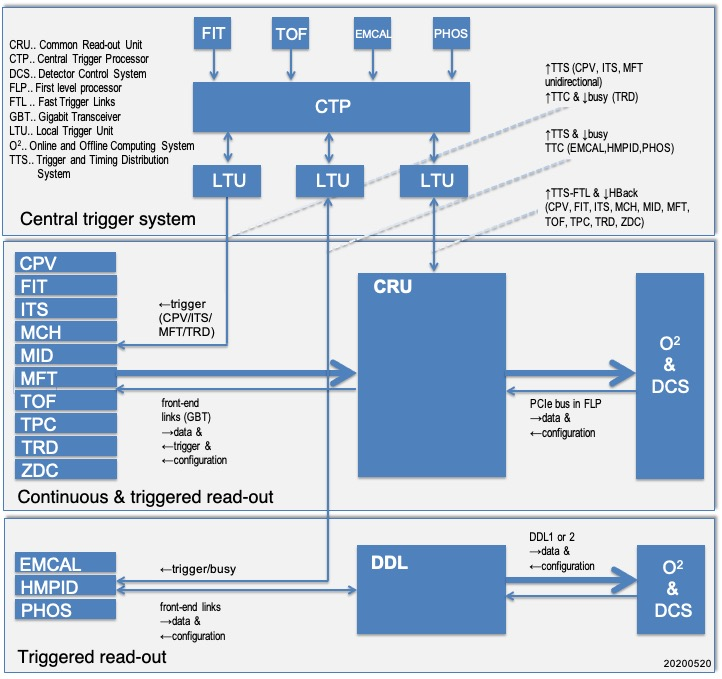
\includegraphics[width=1.\textwidth]{../fig/cru/ro_architecture.jpg}
  \end{center}
  \caption{ALICE read-out architecture: additional info will be added here@, add FLP and EPN farm}
  \label{fig_ro:ro_architecture}
\end{figure*}

\begin{figure*}[hbtp]
  \begin{center}
    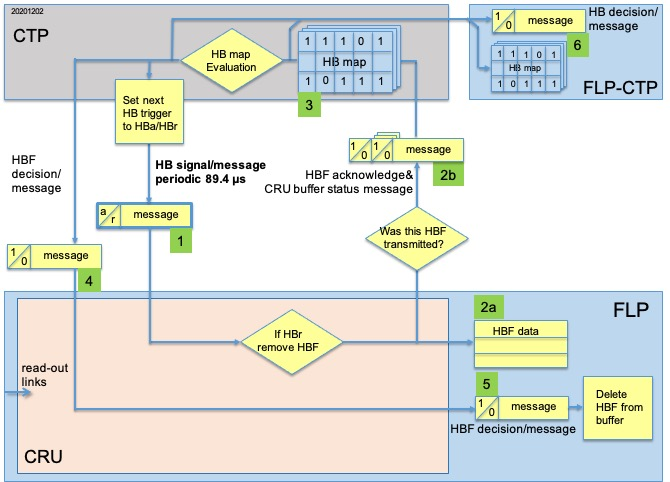
\includegraphics[width=1.\textwidth]{../fig/cru/control_signals.jpg}
  \end{center}
  \caption{ALICE Control signals: additional info will be added here@ or the figure will be removed}
  \label{fig_ro:control_signals}
\end{figure*}





\begin{itemize}
\item Radiation tolerance/load
\item continuous read-out, no filtering but compression (general description), TF and its related impact on reconstruction, CTP-CRU-FLP-EPN approach, implementation specification (beam, particle load, radiation load)
\item beam pipe
\item installation sequence, maintainability of ITS
\end{itemize}


\section{common (chip) developments}
\subsection{ALPIDE}
\subsection{SAMPA}

\section{detector upgrades}
(aim for similar substructure for all detectors)

\begin{figure}
\centering
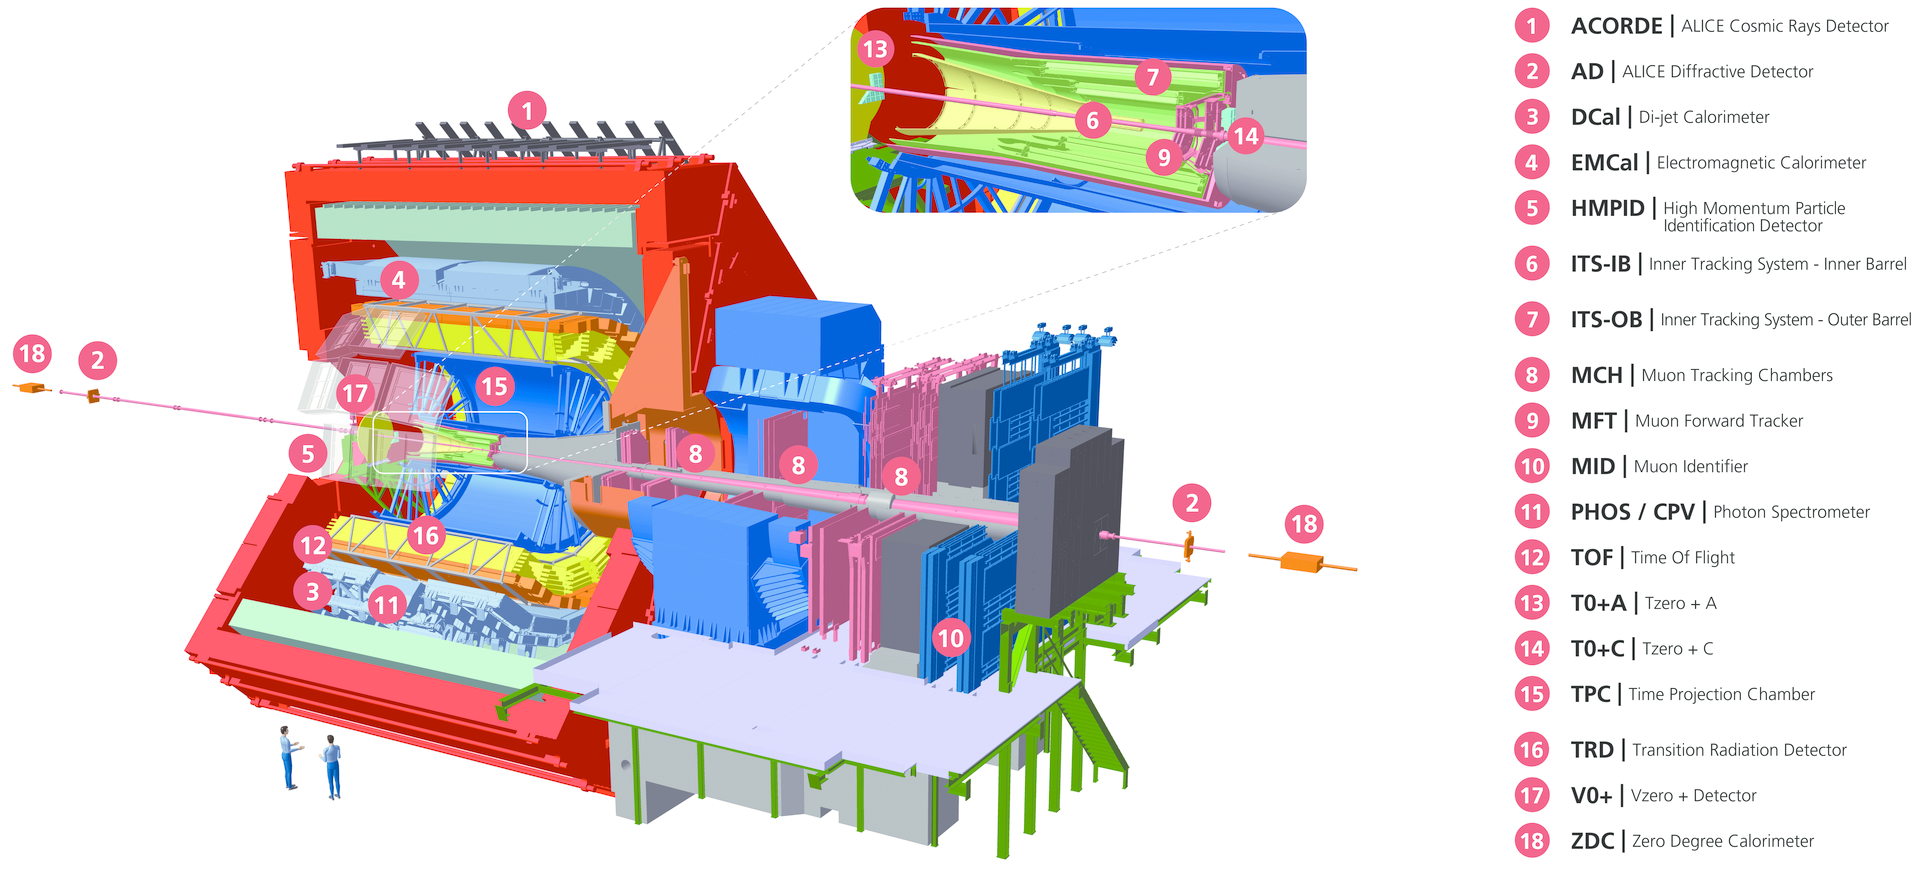
\includegraphics[width=.5\textwidth]{common/2017-May-11-ALICE_RUN3_labels_HD}
\caption{Overview Run 3}
\label{fig:alice_run3}
\end{figure}

\subsection{ITS}
\subsection{MFT}
\subsection{TPC}
\subsection{FIT}
\subsection{Muon System}
\subsection{TRD}
\subsection{TOF}
\subsection{HMPID}
\subsection{EMCal}
\subsection{PHOS}

\section{Beampipe, support structures, detector alignment, installation and maintenance}

\section{read-out and data processing}
\subsection{O2 Overview: reconstruction workflow (PDP)}
(TF structure, …)
\subsection{CTP}
\subsection{CRU}
\subsection{FLP}
\subsection{EPN (hardware/infra)}
\subsection{Grid computing / Offline computing infrastructure}

\section{conclusions}
\subsection{prospects for Run 3 + 4 (expected performance)}

\cleardoublepage
%%%%% acknowledgements - handled by EB chairs
\newenvironment{acknowledgement}{\relax}{\relax}
\begin{acknowledgement}
\section*{Acknowledgements}
% add specific acknowledgements here
% ...but please don't remove the line below: funding agencies
% will be acknowledged with a custom tex file handled by EB chairs after Collab Round 2
%\input{acknowledgements.tex}
\end{acknowledgement}

%%%%%%%% Bibliography
\bibliographystyle{utphys}   % Remember we use title in the biblio
\bibliography{bibliography}
%\input {bibliography.tex}

%%%%%%%%%%%%%%%%%%%%%%%%%%%%%%%%
% Appendices: yours (if any) + authorlist
%%%%%%%%%%%%%%%%%%%%%%%%%%%%%%%%
\newpage
\appendix

%
%\input{} % put your appendices here (if any)
%

%%%%% Authorlist - please do not touch: handled by EB chairs
\section{The ALICE Collaboration}
\label{app:collab}
%\input{authorlist-preprint.tex}
\end{document}
